\section{Componenti utilizzati}
Il progetto si basa su specifici componenti hardware:
\begin{itemize}
  \item Microcontrollore STM32WL55JC, con protocollo multi-modulation radio LoRa
  \item Scheda Multi-Sensor X-NUCLEO-IKS01A3, per l'acqusizione dei sensori
        \begin{itemize}
          \item Accelerometro e giroscopio con misurazione a 3 assi LSM6DSO
        \end{itemize}
\end{itemize}
\begin{figure}[h!]
  \centering
  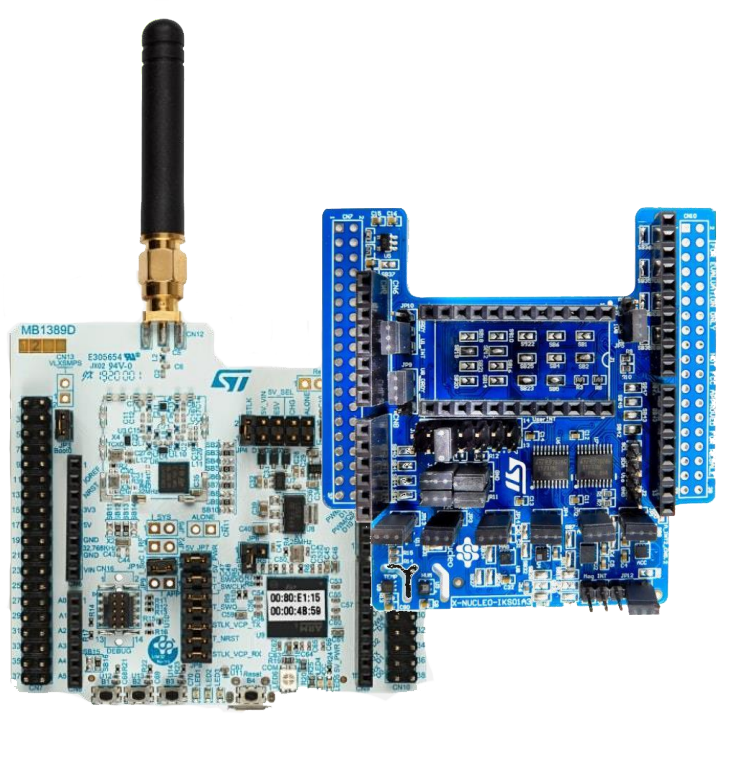
\includegraphics[width=7cm]{schede.png}
  \caption{STM32WL55JC e X-NUCLEO-IKS01A3}
\end{figure}
Si utilizzano inoltre ulteriori componenti software:
\begin{itemize}
  \item STM32CubeIDE per la scrittura del codice C riguardante il Microcontrollore
  \item Ambiente di sviluppo per il codice python riguradante il client
  \item Librerie di supporto pygame e mqtt per l'elaborazione grafica e per la connessione con il cloud
\end{itemize}


